\chapter{Introduction}
\label{ch:intro}
\pagenumbering{arabic}

The increasing popularity and the intensive usage of computational systems in the everyday of modern life creates the need for easier and less invasive forms of authentication. While enter a hard to memorize password in a terminal still is the safest approach, voice biometrics presents itself as a continuing improvement alternative. Also, speech is the most natural way humans have to communicate, being incredibly complex and with numerous specific details related to the speaker \cite{bimbot.et.al.2004}. Therefore, it is expected an increasing usage of vocal interfaces to perform actions such as computer login, voice search (e.g., Apple Siri, Google Now and Samsung S Voice) and identification of speakers in a conversation and its content.

At present, fingerprint biometrics is adopted in several solutions (e.g., ATMs \cite{wang.wu.2002}), authentication through facial recognition comes as built-in software for average computers and iris scan was adopted for a short time by United Kingdom and permanently by United Arab Emirates border controls \cite{sasse.2007, raisi.khouri.2008}. That said, improvements in voice recognition techniques indicate a near future where vocal commands will be used for authentication, alone or combined with other biometric methods.

Current commercial products based on voice technology (e.g., Dragon Naturally Speaking, KIVOX and VeriSpeak) are usually intended to perform either \textbf{speech recognition} (\emph{what} is being said) or \textbf{speaker recognition} (\emph{who} is speaking). Voice search applications are designed to determine the content of a speech, usually with no concern about who the speaker is or if there is more than one, while computer login and telephone fraud prevention supplement a memorized personal identification code with speaker verification \cite{reynolds.1995a}, with no interest on the message spoken. Few applications perform both processes, such as automatic speaker labeling of recorded meetings, that transcribes what each person is saying. To achieve this goal, numerous voice processing techniques have become known in industry and academy, e.g., Natural Language Processing (NLP), Hidden Markov Models (HMMs) and Gaussian Mixture Models (GMMs). Although all of these are interesting state-of-the-art techniques, the subject covered by this paper is a subarea of speaker recognition and only a small subset of these techniques will be unraveled.

\section{Speaker Recognition}
\label{sec:speaker-recognition}

As stated in \cite{reynolds.campbell.2008}, speaker recognition may be divided in two subareas. The first is \textbf{speaker identification}, aimed to determine the identity of a speaker from a non-unitary set of known speakers. This task is also named speaker identification in \textbf{closed set}. In the second, \textbf{speaker verification}, the goal is to determine if a speaker is who he or she claims to be, not an imposter. As the set of imposters is unknown, this is an \textbf{open set} problem. An intermediate task is \textbf{open set identification}, when an ``unmatched class" is added in order to categorize all unknown speakers.

\begin{figure}[ht]
    \centering
    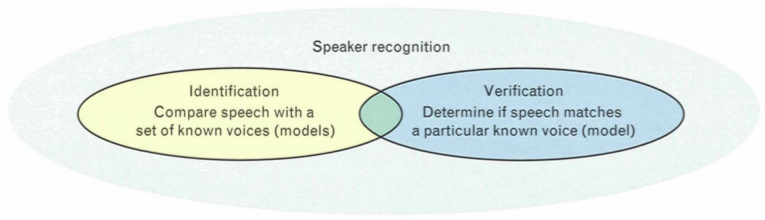
\includegraphics[width=\textwidth]{speaker-recognition}
    \caption{Speaker identification and speaker verification are different, but not entirely \cite{reynolds.1995a}.}
    \label{fig:speaker-recognition}
\end{figure}

The text used may be constrained, such as by type (e.g., digits and letters) and/or by number of words used (e.g., one word or sentences). In \textbf{text-dependent} systems the content of the speech is relevant to the evaluation, and the testing texts must belong to the training set (not necessarily be the entire set) \cite{hebert.2008}. A change in the training text demands an entirely new training section. \textbf{Text-independent} systems have no restrictions to the message in both sets, with the non-textual characteristics of the user's voice (e.g., pitch and accent) being the important aspects to the evaluator. These characteristics are presented in different sentences, usage of different languages and even in gibberish for a speaker. Between the extremes in constraints falls the \textbf{vocabulary-dependent system}, which constrains the speech to come from a limited vocabulary (e.g., digits) from which test words or phrases are selected (e.g., ``two" or ``one-two-three") \cite{reynolds.1995a}.

This paper is focused in \textbf{text-independent speaker verification}, in other words, the acceptance or rejection of a user's claimed identity by analysis of his or her vocal characteristics with no specific text. To achieve that, a speaker's GMM adapted from an Universal Background Model (UBM) \cite{reynolds.quatieri.dunn.2000} is implemented. Also, an adaptation of the technique is proposed and evaluated using Fractional Covariance Matrix (FCM) \cite{gao.zhou.pu.2013}.

\section{Objectives}

The objectives of this study are:

\begin{itemize}\itemsep0pt
    \item Analyze and evaluate the speaker verification system using the adapted GMM seen in \cite{reynolds.quatieri.dunn.2000};
    \item Propose and evaluate a new method derived from GMM, using the FCM theory seen in \cite{gao.zhou.pu.2013};
    \item Conduct experiments for the existent and the proposed methods and perform comparisons.
\end{itemize}

\section{Document Structure}

Chapter 2 contains basic information about voice recognition, as well as the basic architecture for a speaker verification system. The feature extraction process is explained in chapter 3, from the reasons for its use to the chosen technique (Mel-Frequency Cepstral Coefficient, MFCC). In chapter 4 is detailed the GMM and the UBM. Chapter 5 introduces FCM and the proposed Fractional Gaussian Mixture Model (FGMM). Experiments are described in chapter 6, as well as its results. Finally, chapter 7 concludes the study. Furthermore, this work contains an appendix with the most relevant pieces of the source code and some necessary mathematical concepts.